\documentclass[]{article}
\usepackage{lmodern}
\usepackage{amssymb,amsmath}
\usepackage{ifxetex,ifluatex}
\usepackage{bm}
\usepackage{soul}
\usepackage[color=yellow]{todonotes}
\usepackage{fixltx2e} % provides \textsubscript
\ifnum 0\ifxetex 1\fi\ifluatex 1\fi=0 % if pdftex
  \usepackage[T1]{fontenc}
  \usepackage[utf8]{inputenc}
\else % if luatex or xelatex
  \ifxetex
    \usepackage{mathspec}
  \else
    \usepackage{fontspec}
  \fi
  \defaultfontfeatures{Ligatures=TeX,Scale=MatchLowercase}
\fi
% use upquote if available, for straight quotes in verbatim environments
\IfFileExists{upquote.sty}{\usepackage{upquote}}{}
% use microtype if available
\IfFileExists{microtype.sty}{%
\usepackage{microtype}
\UseMicrotypeSet[protrusion]{basicmath} % disable protrusion for tt fonts
}{}
\usepackage[margin=1in]{geometry}
\usepackage{hyperref}
\hypersetup{unicode=true,
            pdftitle={2 Time series models, trend and autocovariance},
            pdfauthor={Edward Ionides},
            pdfborder={0 0 0},
            breaklinks=true}
\urlstyle{same}  % don't use monospace font for urls
\usepackage{color}
\usepackage{fancyvrb}
\newcommand{\VerbBar}{|}
\newcommand{\VERB}{\Verb[commandchars=\\\{\}]}
\DefineVerbatimEnvironment{Highlighting}{Verbatim}{commandchars=\\\{\}}
% Add ',fontsize=\small' for more characters per line
\usepackage{framed}
\definecolor{shadecolor}{RGB}{248,248,248}
\newenvironment{Shaded}{\begin{snugshade}}{\end{snugshade}}
\newcommand{\KeywordTok}[1]{\textcolor[rgb]{0.13,0.29,0.53}{\textbf{#1}}}
\newcommand{\DataTypeTok}[1]{\textcolor[rgb]{0.13,0.29,0.53}{#1}}
\newcommand{\DecValTok}[1]{\textcolor[rgb]{0.00,0.00,0.81}{#1}}
\newcommand{\BaseNTok}[1]{\textcolor[rgb]{0.00,0.00,0.81}{#1}}
\newcommand{\FloatTok}[1]{\textcolor[rgb]{0.00,0.00,0.81}{#1}}
\newcommand{\ConstantTok}[1]{\textcolor[rgb]{0.00,0.00,0.00}{#1}}
\newcommand{\CharTok}[1]{\textcolor[rgb]{0.31,0.60,0.02}{#1}}
\newcommand{\SpecialCharTok}[1]{\textcolor[rgb]{0.00,0.00,0.00}{#1}}
\newcommand{\StringTok}[1]{\textcolor[rgb]{0.31,0.60,0.02}{#1}}
\newcommand{\VerbatimStringTok}[1]{\textcolor[rgb]{0.31,0.60,0.02}{#1}}
\newcommand{\SpecialStringTok}[1]{\textcolor[rgb]{0.31,0.60,0.02}{#1}}
\newcommand{\ImportTok}[1]{#1}
\newcommand{\CommentTok}[1]{\textcolor[rgb]{0.56,0.35,0.01}{\textit{#1}}}
\newcommand{\DocumentationTok}[1]{\textcolor[rgb]{0.56,0.35,0.01}{\textbf{\textit{#1}}}}
\newcommand{\AnnotationTok}[1]{\textcolor[rgb]{0.56,0.35,0.01}{\textbf{\textit{#1}}}}
\newcommand{\CommentVarTok}[1]{\textcolor[rgb]{0.56,0.35,0.01}{\textbf{\textit{#1}}}}
\newcommand{\OtherTok}[1]{\textcolor[rgb]{0.56,0.35,0.01}{#1}}
\newcommand{\FunctionTok}[1]{\textcolor[rgb]{0.00,0.00,0.00}{#1}}
\newcommand{\VariableTok}[1]{\textcolor[rgb]{0.00,0.00,0.00}{#1}}
\newcommand{\ControlFlowTok}[1]{\textcolor[rgb]{0.13,0.29,0.53}{\textbf{#1}}}
\newcommand{\OperatorTok}[1]{\textcolor[rgb]{0.81,0.36,0.00}{\textbf{#1}}}
\newcommand{\BuiltInTok}[1]{#1}
\newcommand{\ExtensionTok}[1]{#1}
\newcommand{\PreprocessorTok}[1]{\textcolor[rgb]{0.56,0.35,0.01}{\textit{#1}}}
\newcommand{\AttributeTok}[1]{\textcolor[rgb]{0.77,0.63,0.00}{#1}}
\newcommand{\RegionMarkerTok}[1]{#1}
\newcommand{\InformationTok}[1]{\textcolor[rgb]{0.56,0.35,0.01}{\textbf{\textit{#1}}}}
\newcommand{\WarningTok}[1]{\textcolor[rgb]{0.56,0.35,0.01}{\textbf{\textit{#1}}}}
\newcommand{\AlertTok}[1]{\textcolor[rgb]{0.94,0.16,0.16}{#1}}
\newcommand{\ErrorTok}[1]{\textcolor[rgb]{0.64,0.00,0.00}{\textbf{#1}}}
\newcommand{\NormalTok}[1]{#1}
\usepackage{graphicx,grffile}
\makeatletter
\def\maxwidth{\ifdim\Gin@nat@width>\linewidth\linewidth\else\Gin@nat@width\fi}
\def\maxheight{\ifdim\Gin@nat@height>\textheight\textheight\else\Gin@nat@height\fi}
\makeatother
% Scale images if necessary, so that they will not overflow the page
% margins by default, and it is still possible to overwrite the defaults
% using explicit options in \includegraphics[width, height, ...]{}
\setkeys{Gin}{width=\maxwidth,height=\maxheight,keepaspectratio}
\IfFileExists{parskip.sty}{%
\usepackage{parskip}
}{% else
\setlength{\parindent}{0pt}
\setlength{\parskip}{6pt plus 2pt minus 1pt}
}
\setlength{\emergencystretch}{3em}  % prevent overfull lines
\providecommand{\tightlist}{%
  \setlength{\itemsep}{0pt}\setlength{\parskip}{0pt}}
\setcounter{secnumdepth}{0}
% Redefines (sub)paragraphs to behave more like sections
\ifx\paragraph\undefined\else
\let\oldparagraph\paragraph
\renewcommand{\paragraph}[1]{\oldparagraph{#1}\mbox{}}
\fi
\ifx\subparagraph\undefined\else
\let\oldsubparagraph\subparagraph
\renewcommand{\subparagraph}[1]{\oldsubparagraph{#1}\mbox{}}
\fi

%%% Use protect on footnotes to avoid problems with footnotes in titles
\let\rmarkdownfootnote\footnote%
\def\footnote{\protect\rmarkdownfootnote}

%%% Change title format to be more compact
\usepackage{titling}

% Create subtitle command for use in maketitle
\newcommand{\subtitle}[1]{
  \posttitle{
    \begin{center}\large#1\end{center}
    }
}

\setlength{\droptitle}{-2em}
  \title{2. Time series models, trend and autocovariance}
  \pretitle{\vspace{\droptitle}\centering\huge}
  \posttitle{\par}
  \author{Edward Ionides}
  \preauthor{\centering\large\emph}
  \postauthor{\par}
  \predate{\centering\large\emph}
  \postdate{\par}
  \date{1/7/2018}


\begin{document}
\maketitle

{
\setcounter{tocdepth}{2}
\tableofcontents
}
\newcommand\E{\mathbb{E}}
\newcommand\prob{\mathbb{P}}
\newcommand\var{\mathrm{Var}}
\newcommand\cov{\mathrm{Cov}}
\newcommand\loglik{\ell}
\newcommand\R{\mathbb{R}}
\newcommand\data[1]{#1^*}
\newcommand\estimate[1]{\data{#1}}
\newcommand\given{\, ; \,}
\newcommand\transpose{\scriptsize{T}}
\newcommand\mycolon{\,{:}\,}





\begin{center}\rule{0.5\linewidth}{\linethickness}\end{center}

\begin{center}\rule{0.5\linewidth}{\linethickness}\end{center}

Objectives

\begin{enumerate}
\def\labelenumi{\arabic{enumi}.}
\item
  Set up general notation for working with time series data and time
  series models.
\item
  Define the trend function for a time series model, and discuss its
  estimation from data. In particular, discuss the properties of least
  square estimation of the trend.
\item
  Define the autocovariance and autocorrelation functions and their
  standard estimators.
\end{enumerate}

\begin{center}\rule{0.5\linewidth}{\linethickness}\end{center}

\begin{center}\rule{0.5\linewidth}{\linethickness}\end{center}

\subsection{Definition: Time series data and time series
models}\label{definition-time-series-data-and-time-series-models}

\begin{itemize}
\item
  A time series is a sequence of numbers, called \textbf{data}. In
  general, we will suppose that there are \(N\) numbers,
  \(\data{y_1},\data{y_2},\dots,\data{y_N}\), collected at an increasing
  sequence of times, \(t_1,t_2,\dots,t_N\).

  \begin{itemize}
  \item
    We write \(1{\mycolon}N\) for the sequence \(\{1,2,\dots,N\}\) and
    we write the collection of numbers \(\{\data{y_n}, n=1,\dots,N\}\)
    as \(\data{y_{1:N}}\).
  \item
    We keep \(t\) to represent continuous time, and \(n\) to represent
    the discrete sequence of observations. This will serve us well
    later, when we fit continuous time models to data.
  \end{itemize}
\item
  \hl{A time series model is a collection of jointly defined random
  variables, $Y_1,Y_2,\dots,Y_N$.}

  \begin{itemize}
  \item
    We write this collection of random variables as \(Y_{1:N}\).
  \item
    Like all jointly defined random variables, the distribution of
    \(Y_{1:N}\) is defined by a joint density function, which we write
    as \[ f_{Y_{1:N}}(y_1,\dots,y_N \given \theta).\]
  \item
    Here, \(\theta\) is a vector of parameters.
  \item
    This notation generalizes. We will generally write \(f_Y(y)\) for
    the density of a random variable \(Y\) evaluated at \(y\), and
    \(f_{YZ}(y,z)\) for the joint density of the pair of random
    variables \((Y,Z)\) evaluated at \((y,z)\). We can also write
    \(f_{Y|Z}(y|z)\) for the conditional density of \(Y\) given \(Z\).
  \item
    For discrete data, such as count data, our model may also be
    discrete and we interpret the density function as a probability mass
    function. Formulas for expectations and probabilities are written as
    integrals for continuous models, and sums for discrete models.
    Otherwise, everything remains the same. We will write formulas only
    for the continuous case. You should be able to swap integrals for
    sums, if necessary, to work with discrete models.
  \item
    Scientifically, we postulate that \(\data{y_{1:N}}\) are a
    realization of \(Y_{1:N}\) for some unknown value of \(\theta\).
  \end{itemize}
\item
  Our notation distinguishes between

  \begin{itemize}
  \tightlist
  \item
    the model, \(Y_{1:N}\)
  \item
    an arbitrary realization of the model, \(y_{1:N}\)
  \item
    the specific sequence of numbers that we observed as data,
    \(\data{y_{1:N}}\)
  \end{itemize}
\end{itemize}

\begin{center}\rule{0.5\linewidth}{\linethickness}\end{center}

\begin{center}\rule{0.5\linewidth}{\linethickness}\end{center}

\subsubsection{Review questions}\label{review-questions}

\begin{enumerate}
\def\labelenumi{\arabic{enumi}.}
\item
  What is a random variable?
\item
  What is a collection of jointly defined random variables?
\item
  What is a probability density function? What is a joint density
  function? What is a conditional density function?
\item
  What does it mean to say that ``\(\theta\) is a vector of
  parameters?''
\end{enumerate}

(There are different answers to these questions, but you should be able
to write down an answer that you are satisfied with.)

\begin{center}\rule{0.5\linewidth}{\linethickness}\end{center}

\begin{center}\rule{0.5\linewidth}{\linethickness}\end{center}

\subsection{Definition: The mean function, or
trend}\label{definition-the-mean-function-or-trend}

\begin{itemize}
\tightlist
\item
  Random variables usually have an expected value, and in this course
  they always do. We write \(\E[X]\) for the expected value of a random
  variable \(X\).
\end{itemize}

\begin{center}\rule{0.5\linewidth}{\linethickness}\end{center}

\subsubsection{Review question}\label{review-question}

What is expected value? How is it defined? How can it fail to exist for
a properly defined random variable?

\begin{center}\rule{0.5\linewidth}{\linethickness}\end{center}

\begin{itemize}
\item
  We define the \textbf{mean function} by
  \[ \mu_n = \E[Y_n] = \int_{-\infty}^\infty y_n \, f^{}_{Y_n}(y_n)\, dy_n\]
  for \(n\in 1{\mycolon}N\).
\item
  We use the words ``mean function'' and ``trend'' interchangeably.
\item
  We say ``function'' since we are thinking of \(\mu_n\) as a function
  of \(n\).

  \begin{itemize}
  \item
    Sometimes, it makes sense to think of \hl{time as continuous}. Then, we
    can write \[\mu(t)\] for the expected value of an observation at
    time \(t\). \hl{We only make observations at the discrete collection of
    times $t_{1:N}$} and so we require $$\mu(t_n)= \mu_n.$$
  \item
    A time series may have measurements evenly spaced in time, but our
    notation does not insist on this. In practice, time series data may
    contain missing values or unequally spaced observations.
  \end{itemize}
\item
  \(\mu_n\) may depend on \(\theta\), the parameter vector. We can write
  \(\mu_n(\theta)\) to make this explicit.
\item
  We \hl{write $\hat\mu_n(y_{1:N})$ to be some estimator of $\mu_n$,
  i.e., a map which is applied to the data to give an estimate of
  $\mu_n$}. An appropriate choice of \(\hat\mu_n\) will depend on the
  data and the model.
  
  \todo[inline]{Difference b/t estimators and estimates. Estimators are functions of arbitrary realizations of random variables. Estimates are real numbers (data) subbed in for these arbitrary values within the estimators.}
\item
  Usually, applied statistics courses do not distinguish between
  estimators (functions that can be applied to any dataset) and
  estimates (an estimator evaluated on the actual data). In this course,
  we will want to be quite careful when thinking about model
  specification and diagnosing model misspecification. Therefore, we are
  going to try to preserve this distinction. Properly, this distinction
  is always there, but is often ignored.
\item
  For example, the estimate of the mean function is the value of the
  estimator when applied to the data. Here, we write this as
  \[ \data{\hat\mu_n} = \hat\mu_n(\data{y_{1:N}}).\]
\item
  We call \(\data{\hat\mu_n}\) an \textbf{estimated mean function} or
  \hl{\textbf{estimated trend}}.
  \todo[inline]{Saying ``the data have a trend'' implies that a model with a non-constant mean-function seems appropriate. Or, in other words, ``within a model class M, only models with trend well describe the data''}
\item
  For example, \hl{sometimes we suppose a model with $\mu_n=\mu$, so the
  mean is assumed constant}. In this case, the \hl{model is called
  \textbf{mean stationary}}. Then, we might \hl{estimate $\mu$ using the
  mean estimator,} \[\hat\mu(y_{1:N})=\frac{1}{N}\sum_{k=1}^N y_k.\] In
  this case, the corresponding estimate
  \(\data{\hat\mu}=\hat\mu(\data{y_{1:N}})\) is the sample mean.

  \begin{itemize}
  \item
    We can compute the sample mean, \(\data{\hat\mu}\), for any dataset.
    It is only a reasonable estimator of the mean function when a mean
    stationary model is appropriate.
  \item
    Notice that trend is a property of the model, and the estimated
    trend is a function of the data.
  \item
    Formally, we should not talk about the trend of the data. People do,
    but we should try not to.
  \item
    Similarly, data cannot be mean stationary. A model can be mean
    stationary.
  \end{itemize}
\end{itemize}

\begin{center}\rule{0.5\linewidth}{\linethickness}\end{center}

\subsubsection{Question: properties of models vs properties of
data}\label{question-properties-of-models-vs-properties-of-data}

Consider these two statements. Does is matter which we use?

\begin{verbatim}
    1. ``The data look mean stationary.''

    2. ``A mean stationary model looks appropriate for these data.''
\end{verbatim}

\begin{center}\rule{0.5\linewidth}{\linethickness}\end{center}

\begin{center}\rule{0.5\linewidth}{\linethickness}\end{center}

\subsection{Definition: The autocovariance and autocorrelation
functions, and some estimators of
them}\label{definition-the-autocovariance-and-autocorrelation-functions-and-some-estimators-of-them}

\begin{itemize}
\item
  We will assume that variances and covariances exist for the random
  variables \(Y_{1:N}\). We write
  \[ \gamma_{m,n} = \E\big[(Y_m-\mu_m)(Y_n-\mu_n)\big].\] This is called
  the \hl{\textbf{autocovariance} function}, viewed as a function of \(m\)
  and \(n\).
\item
  We may also write \(\Gamma\) for the matrix whose \((m,n)\) entry is
  \(\gamma_{m,n}\).
\item
  Often, we will \hl{suppose that the covariance between two observations
  depends only on the time difference between the observations}. In this
  case, we say that the time series model is \hl{\textbf{covariance
  stationary}}. Supposing also that the observations are equally spaced
  in time, we write the autocovariance function as a function of a lag,
  \(h\), given by \[ \gamma_{h} = \gamma_{n,n+h}.\]
\item
  For a covariance stationary model, and some mean function estimator
  \(\hat\mu_n=\hat \mu_n(y_{1:N})\), a common estimator for \(\gamma_h\)
  is
  \[ \hat\gamma_h(y_{1:N}) = \frac{1}{N}\sum_{n=1}^{N-h} \big( {y_n} - \hat\mu_n \big)\, \big({y_{n+h}}-\hat\mu_{n+h} \big).\]
\item
  The corresponding estimate of \(\gamma_h\), known as the
  \textbf{sample autocovariance function}, is
  \[\data{\hat\gamma_h} = \hat\gamma_h(\data{y_{1:N}}).\]
\item
  Dividing the autocovariance by the variance gives the
  \textbf{autocorrelation function} \(\rho_h\) given by
  \[ \rho_h = \frac{\gamma_h}{\gamma_0}.\] We can analogously construct
  the standard autocorrelation estimator,
  \[ \hat\rho_h(y_{1:N}) = \frac{\hat\gamma_h(y_{1:N})}{\hat\gamma_0(y_{1:N})},\]
  which leads to an estimate known as the \textbf{sample
  autocorrelation},
  \[ \data{\hat\rho_h} = \hat\rho_h(\data{y_{1:N}})= \frac{\data{\hat\gamma_h}}{\data{\hat\gamma_0}}.\]
\item
  It is common to use ACF as an acronym for any or all of the
  autocorrelation function, sample autocorrelation function,
  autocovariance function, and sample autocovariance function.
  \hl{\textbf{If you use the acronym ACF, you are expected to define it, to
  remove the ambiguity}.}
\item
  The sample autocorrelation and sample autocovariance functions are
  statistics computed from the data. They exist, and can be computed,
  even when the data are not well modeled as covariance stationary.
  However, in that case, it does not make sense to view them as
  estimators of the autocorrelation and autocovariance functions (which
  exist as functions of a lag \(h\) only for covariance stationary
  models).
\item
  Formally, we should not talk about the correlation or covariance of
  data. These are properties of models. We can talk about the sample
  autocorrelation or sample autocovariance of data.
\end{itemize}

\begin{center}\rule{0.5\linewidth}{\linethickness}\end{center}

\begin{center}\rule{0.5\linewidth}{\linethickness}\end{center}

\subsection{Estimating a trend by least
squares}\label{estimating-a-trend-by-least-squares}

Let's analyze a time series of global mean annual temperature downloaded
from
\url{http://climate.nasa.gov/system/internal_resources/details/original/647_Global_Temperature_Data_File.txt}.
These data are in degrees Celsius measured as an anomaly from a
1951-1980 base. This is climatology jargon for saying that the sample
mean of the temperature over the interval 1951-1980 was subtracted from
all time points.

\begin{Shaded}
\begin{Highlighting}[]
\NormalTok{global_temp <-}\StringTok{ }\KeywordTok{read.table}\NormalTok{(}\StringTok{"Global_Temperature.txt"}\NormalTok{,}\DataTypeTok{header=}\OtherTok{TRUE}\NormalTok{)}
\KeywordTok{str}\NormalTok{(global_temp)}
\end{Highlighting}
\end{Shaded}

\begin{verbatim}
## 'data.frame':    137 obs. of  3 variables:
##  $ Year            : int  1880 1881 1882 1883 1884 1885 1886 1887 1888 1889 ...
##  $ Annual          : num  -0.2 -0.12 -0.1 -0.21 -0.28 -0.32 -0.31 -0.33 -0.2 -0.12 ...
##  $ Moving5yrAverage: num  -0.13 -0.16 -0.19 -0.21 -0.24 -0.26 -0.27 -0.27 -0.27 -0.26 ...
\end{verbatim}

\begin{Shaded}
\begin{Highlighting}[]
\KeywordTok{plot}\NormalTok{(Annual}\OperatorTok{~}\NormalTok{Year,}\DataTypeTok{data=}\NormalTok{global_temp,}\DataTypeTok{ty=}\StringTok{"l"}\NormalTok{)}
\end{Highlighting}
\end{Shaded}

\begin{center}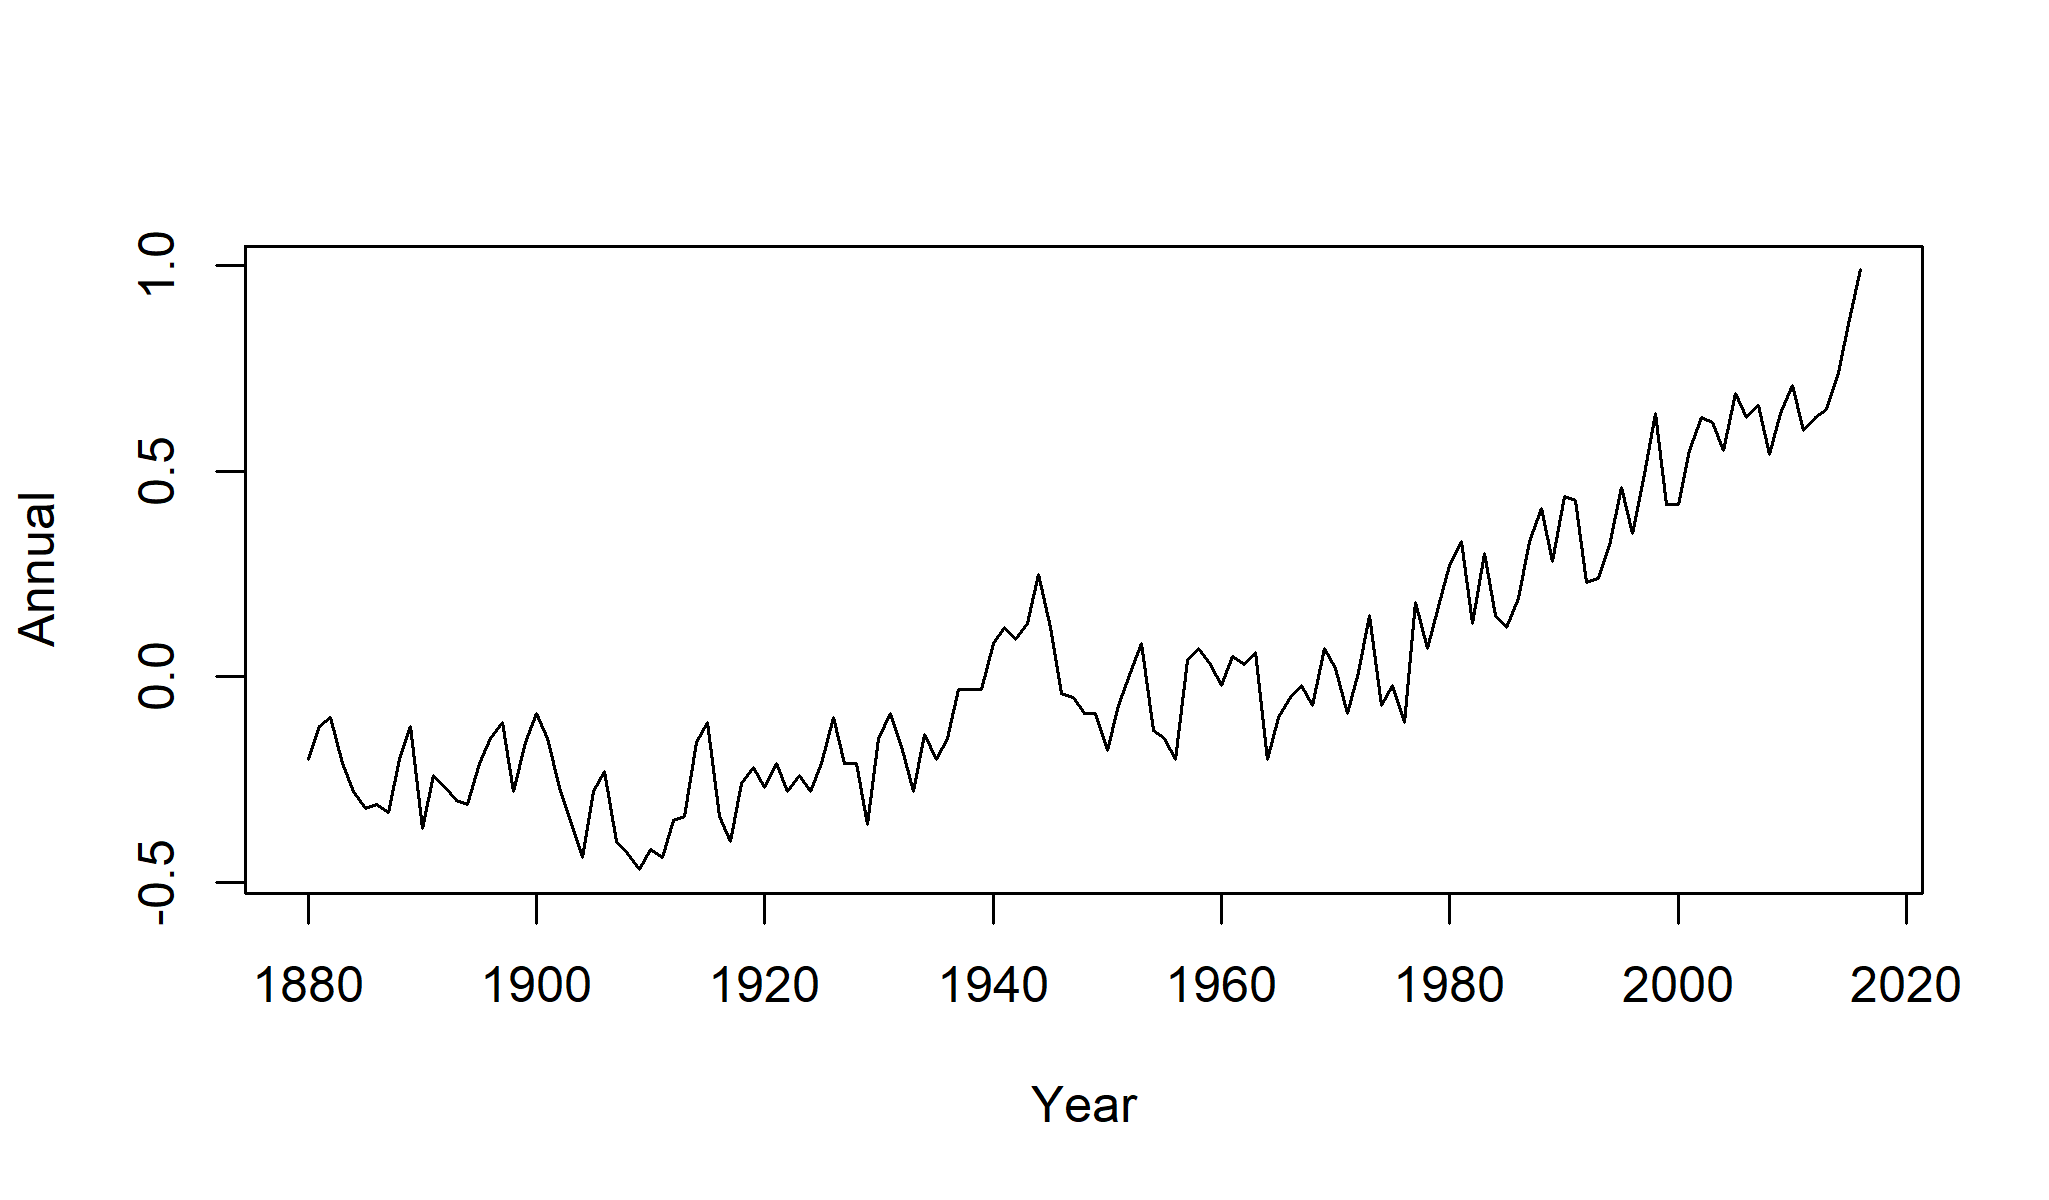
\includegraphics{figure/intro-data_plot-1} \end{center}

\begin{itemize}
\item
  These data should make all of us pause for thought about the future of
  our planet.
\item
  Truly understanding climate change involves understanding the hugely
  complex systems of physical, chemical and biological processes driving
  climate.
\item
  However, it is very hard to know if the gigantic models that attempt
  to capture all important parts of the global climate processes are in
  fact a reasonable description of what is happening.
\item
  There is value in relatively simple statistical analysis, which can at
  least help to tell us what evidence there is for how things are, or
  are not, changing.
\item
  Here is a quote from \emph{Science} (18 December 2015, volume 350,
  page 1461; I've added some emphasis). ``Scientists are still debating
  whether---and, if so, how---warming in the Arctic and dwindling sea
  ice influences extreme weather events at midlatitudes. \textbf{Model
  limitations}, \textbf{scarce data} on the warming Arctic, and the
  \textbf{inherent variability} of the systems make answers elusive.''
\end{itemize}

\subsubsection{Fitting a least squares model with a quadratic
trend}\label{fitting-a-least-squares-model-with-a-quadratic-trend}

Perhaps the simplest trend model that makes sense looking at these data
is a quadratic trend, \[\mu(t)= \beta_0 + \beta_1 t + \beta_2 t^2.\] To
write the least squares estimate of \(\beta_0\), \(\beta_1\) and
\(\beta_2\), we set up matrix notation. Write
\[ \mu = (\mu_1,\mu_2,\dots,\mu_N)^{\transpose}\] for the column vector
describing the mean function, and similarly,
\[ \beta = (\beta_0,\beta_1,\beta_2)^{\transpose}.\] Then, defining
\[ Z = \left(\begin{array}{ccc}
1 & 1880 & 1880^2 \\
1 & 1881 & 1881^2 \\
1 & 1882 & 1882^2 \\
\vdots & \vdots & \vdots
\end{array}\right),\] we have \[ \mu = Z\beta.\] We also write a generic
potential dataset \(y_{1:N}\) and the data \(\data{y_{1:N}}\) as column
vectors,

\begin{eqnarray}
y &=& (y_1,y_2,\dots,y_N)^{\transpose},\\
\data{y} & =& (\data{y_1},\data{y_2},\dots,\data{y_N})^{\transpose}.
\end{eqnarray}

The ordinary least squares (OLS) estimator of \(\beta\) is
\[\hat\beta_{OLS}(y_{1:N}) = (Z^{\transpose} Z)^{-1}Z^{\transpose} y,\]
with corresponding OLS estimate
\[\estimate{\hat\beta}=\hat\beta_{OLS}(\data{y_{1:N}}) = (Z^{\transpose} Z)^{-1}Z^{\transpose} \data{y}.\]
We can carry out this computation in R by

\begin{Shaded}
\begin{Highlighting}[]
\NormalTok{lm_fit <-}\StringTok{ }\KeywordTok{lm}\NormalTok{(Annual}\OperatorTok{~}\NormalTok{Year}\OperatorTok{+}\KeywordTok{I}\NormalTok{(Year}\OperatorTok{^}\DecValTok{2}\NormalTok{),}\DataTypeTok{data=}\NormalTok{global_temp)}
\KeywordTok{summary}\NormalTok{(lm_fit)}
\end{Highlighting}
\end{Shaded}

\begin{verbatim}
## 
## Call:
## lm(formula = Annual ~ Year + I(Year^2), data = global_temp)
## 
## Residuals:
##      Min       1Q   Median       3Q      Max 
## -0.27092 -0.08638  0.00613  0.07481  0.38067 
## 
## Coefficients:
##               Estimate Std. Error t value Pr(>|t|)    
## (Intercept)  2.959e+02  2.681e+01   11.04   <2e-16 ***
## Year        -3.111e-01  2.753e-02  -11.30   <2e-16 ***
## I(Year^2)    8.168e-05  7.067e-06   11.56   <2e-16 ***
## ---
## Signif. codes:  0 '***' 0.001 '**' 0.01 '*' 0.05 '.' 0.1 ' ' 1
## 
## Residual standard error: 0.1157 on 134 degrees of freedom
## Multiple R-squared:  0.8766, Adjusted R-squared:  0.8748 
## F-statistic: 476.1 on 2 and 134 DF,  p-value: < 2.2e-16
\end{verbatim}

where \texttt{I()} is a function that tells R to construct
\texttt{Year\^{}2} as a variable, and inhibits interpretation in the R
model formula notation.

We can check visually how well this model fits the data.

\begin{Shaded}
\begin{Highlighting}[]
\NormalTok{yr <-}\StringTok{ }\DecValTok{1880}\OperatorTok{:}\DecValTok{2026}
\NormalTok{Z <-}\StringTok{ }\KeywordTok{cbind}\NormalTok{(}\DecValTok{1}\NormalTok{,yr,yr}\OperatorTok{^}\DecValTok{2}\NormalTok{)}
\NormalTok{beta <-}\StringTok{ }\KeywordTok{coef}\NormalTok{(lm_fit)}
\NormalTok{prediction <-}\StringTok{ }\NormalTok{Z}\OperatorTok\NormalTok{beta}
\KeywordTok{plot}\NormalTok{(Annual}\OperatorTok{~}\NormalTok{Year,}\DataTypeTok{data=}\NormalTok{global_temp,}\DataTypeTok{ty=}\StringTok{"l"}\NormalTok{,}\DataTypeTok{xlim=}\KeywordTok{range}\NormalTok{(yr),}\DataTypeTok{ylim=}\KeywordTok{range}\NormalTok{(}\KeywordTok{c}\NormalTok{(global_temp}\OperatorTok{\$}\NormalTok{Annual,prediction),}\DataTypeTok{na.rm=}\OtherTok{TRUE}\NormalTok{),}\DataTypeTok{lty=}\StringTok{"dashed"}\NormalTok{)}
\KeywordTok{lines}\NormalTok{(}\DataTypeTok{x=}\NormalTok{yr,}\DataTypeTok{y=}\NormalTok{prediction,}\DataTypeTok{col=}\StringTok{"red"}\NormalTok{)}
\end{Highlighting}
\end{Shaded}

\begin{center}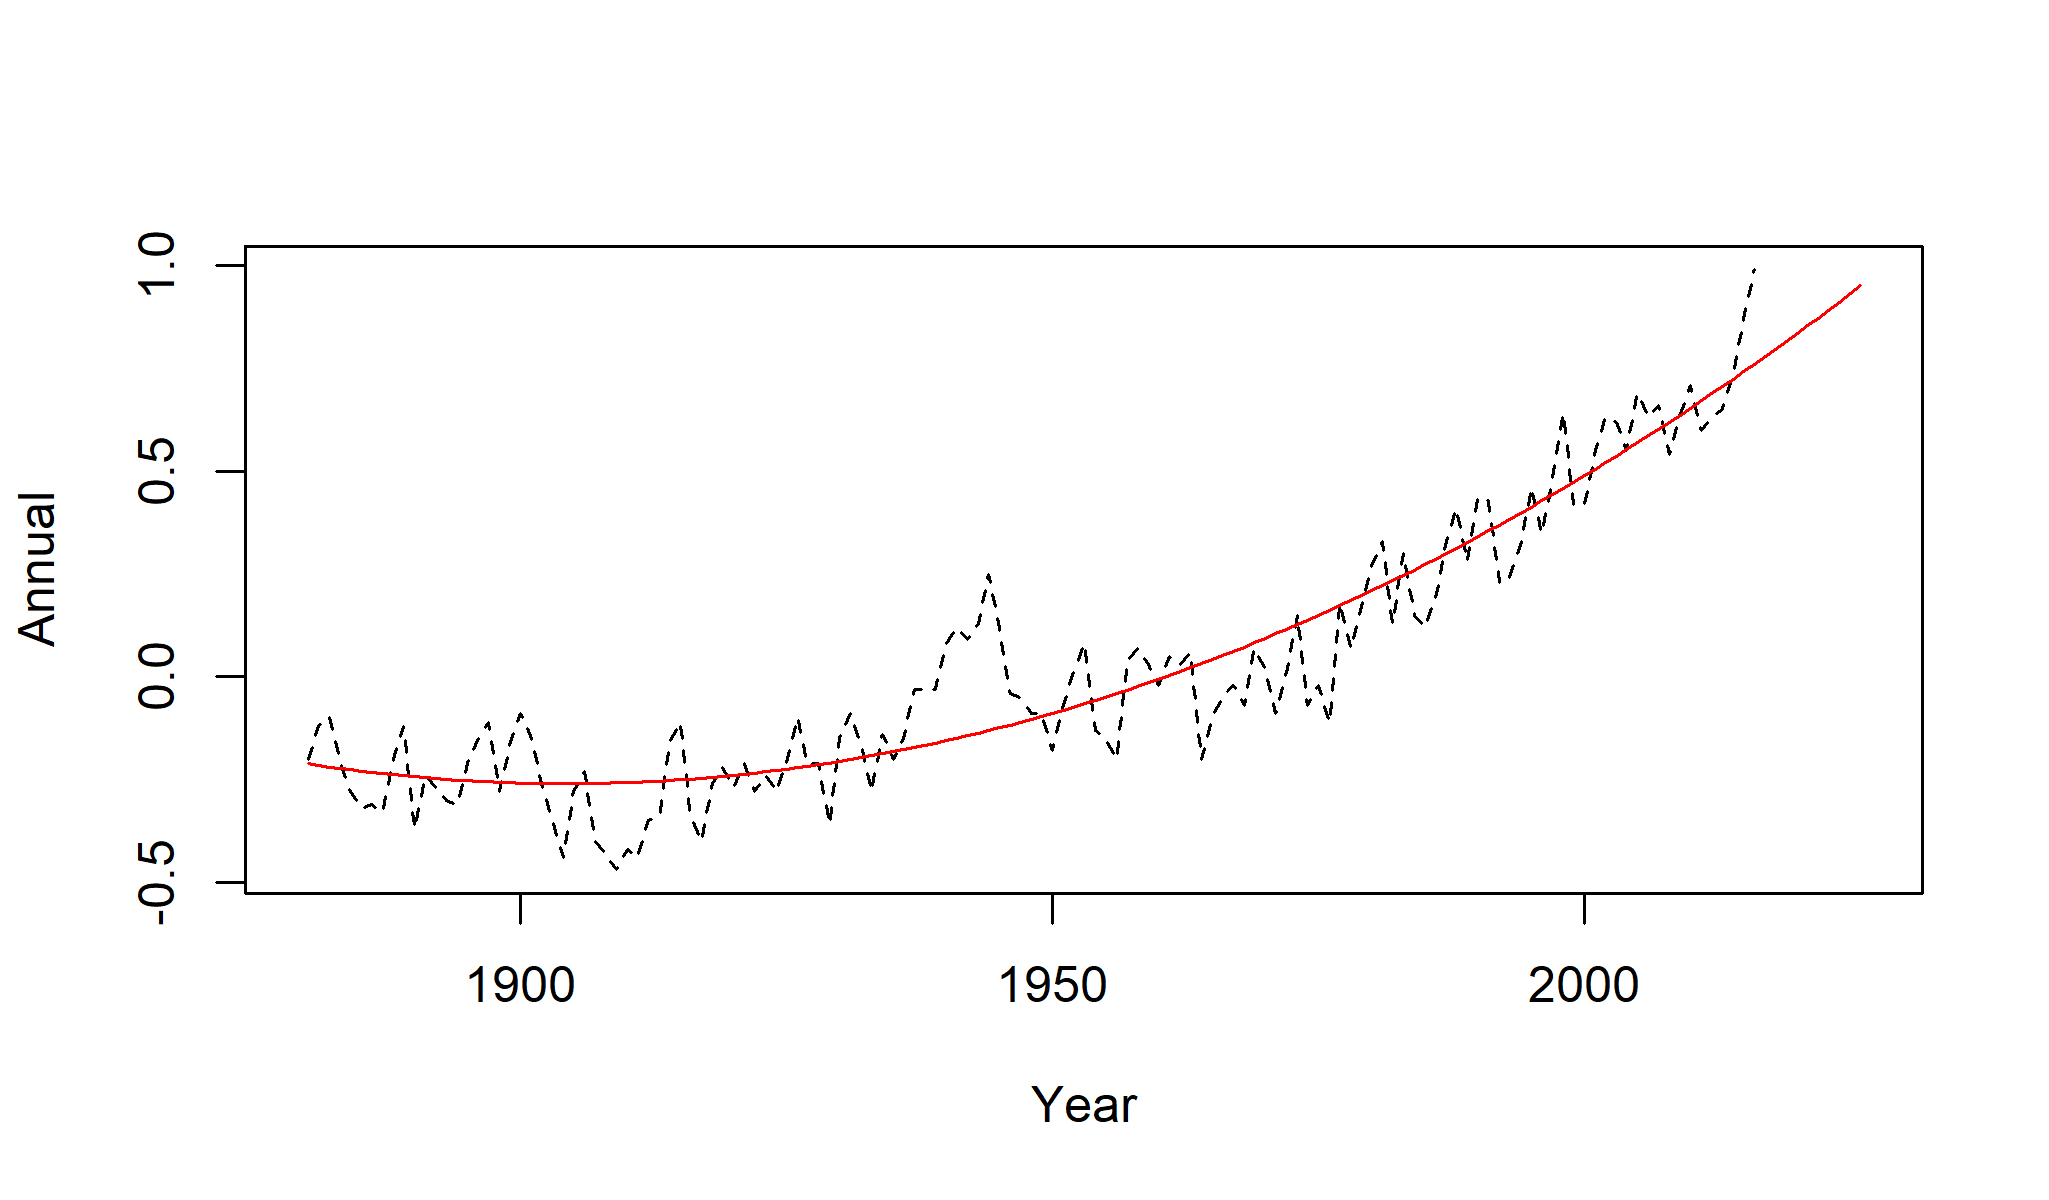
\includegraphics{figure/intro-glob_temp_lm_plot-1} \end{center}

\begin{itemize}
\item
  The overall estimated trend seems a reasonable fit for the data.
\item
  If we want to attach uncertainty to our parameter estimates, and
  consequently to our forecast, we need a time series model \(Y_{1:N}\),
  which we write in column vector form as
  \[Y = (Y_1,Y_2,\dots,Y_N)^{\transpose}.\]
\item
  The standard OLS model is $${[}L1{]}
  \quad\quad\quad\quad\quad Y = Z\beta + \epsilon,$$ where
  \(\epsilon=\epsilon_{1:N}\) is a vector of independent, identically
  distributed random variables with mean zero and constant variance,
  \[\E[\epsilon_n]=0, \quad\quad \var[\epsilon_n] = \sigma^2.\] Standard
  linear model software, such as \texttt{lm} in R, provides confidence
  intervals based on this model.
\item
  Under model L1, the estimator \(\hat\beta_{OLS}(y_{1:N})\) is
  unbiased. This can be checked:

  \begin{eqnarray}
  \E\big[\hat\beta_{OLS}(Y_{1:N})\big] &=&\E\big[ (Z^{\transpose} Z)^{-1}Z^{\transpose} Y \big]\\
  &=& \E\big[ (Z^{\transpose} Z)^{-1}Z^{\transpose} \{Z\beta + \epsilon \}\big]\\
  &=&  (Z^{\transpose} Z)^{-1}Z^{\transpose} \{Z\beta + \E[\epsilon]\} \\
  &=&  (Z^{\transpose} Z)^{-1}(Z^{\transpose} Z)\beta \\
  &=& \beta
  \end{eqnarray}
\item
  A result for linear models is that \(\hat\beta_{OLS}(y_{1:N})\) is the
  minimum variance unbiased estimator for model L1.
\item
  The variance/covariance matrix of \(\hat\beta_{OLS}(Y_{1:N})\) under
  this model is
  \[\cov[\hat\beta_{OLS}(Y_{1:N})] = \sigma^2 \big( Z^{\transpose} Z\big)^{-1},\]
  which is estimated using an estimator for \(\sigma\) of
  \[\hat\sigma_{OLS}(y_{1:N})= \sqrt{\frac{1}{N-d} \big(y-Z\hat\beta_{OLS}\big)^{\transpose} \big(y-Z\hat\beta_{OLS}\big)},\]
  where \(d\) is the number of covariates, i.e., the number of columns
  of \(Z\).
  \todo[inline]{This is the root mean square of the residuals}
\end{itemize}

Let's look at the residuals to assess how appropriate this model is
here.

\begin{Shaded}
\begin{Highlighting}[]
\KeywordTok{acf}\NormalTok{(}\KeywordTok{resid}\NormalTok{(lm_fit))}
\end{Highlighting}
\end{Shaded}

\begin{center}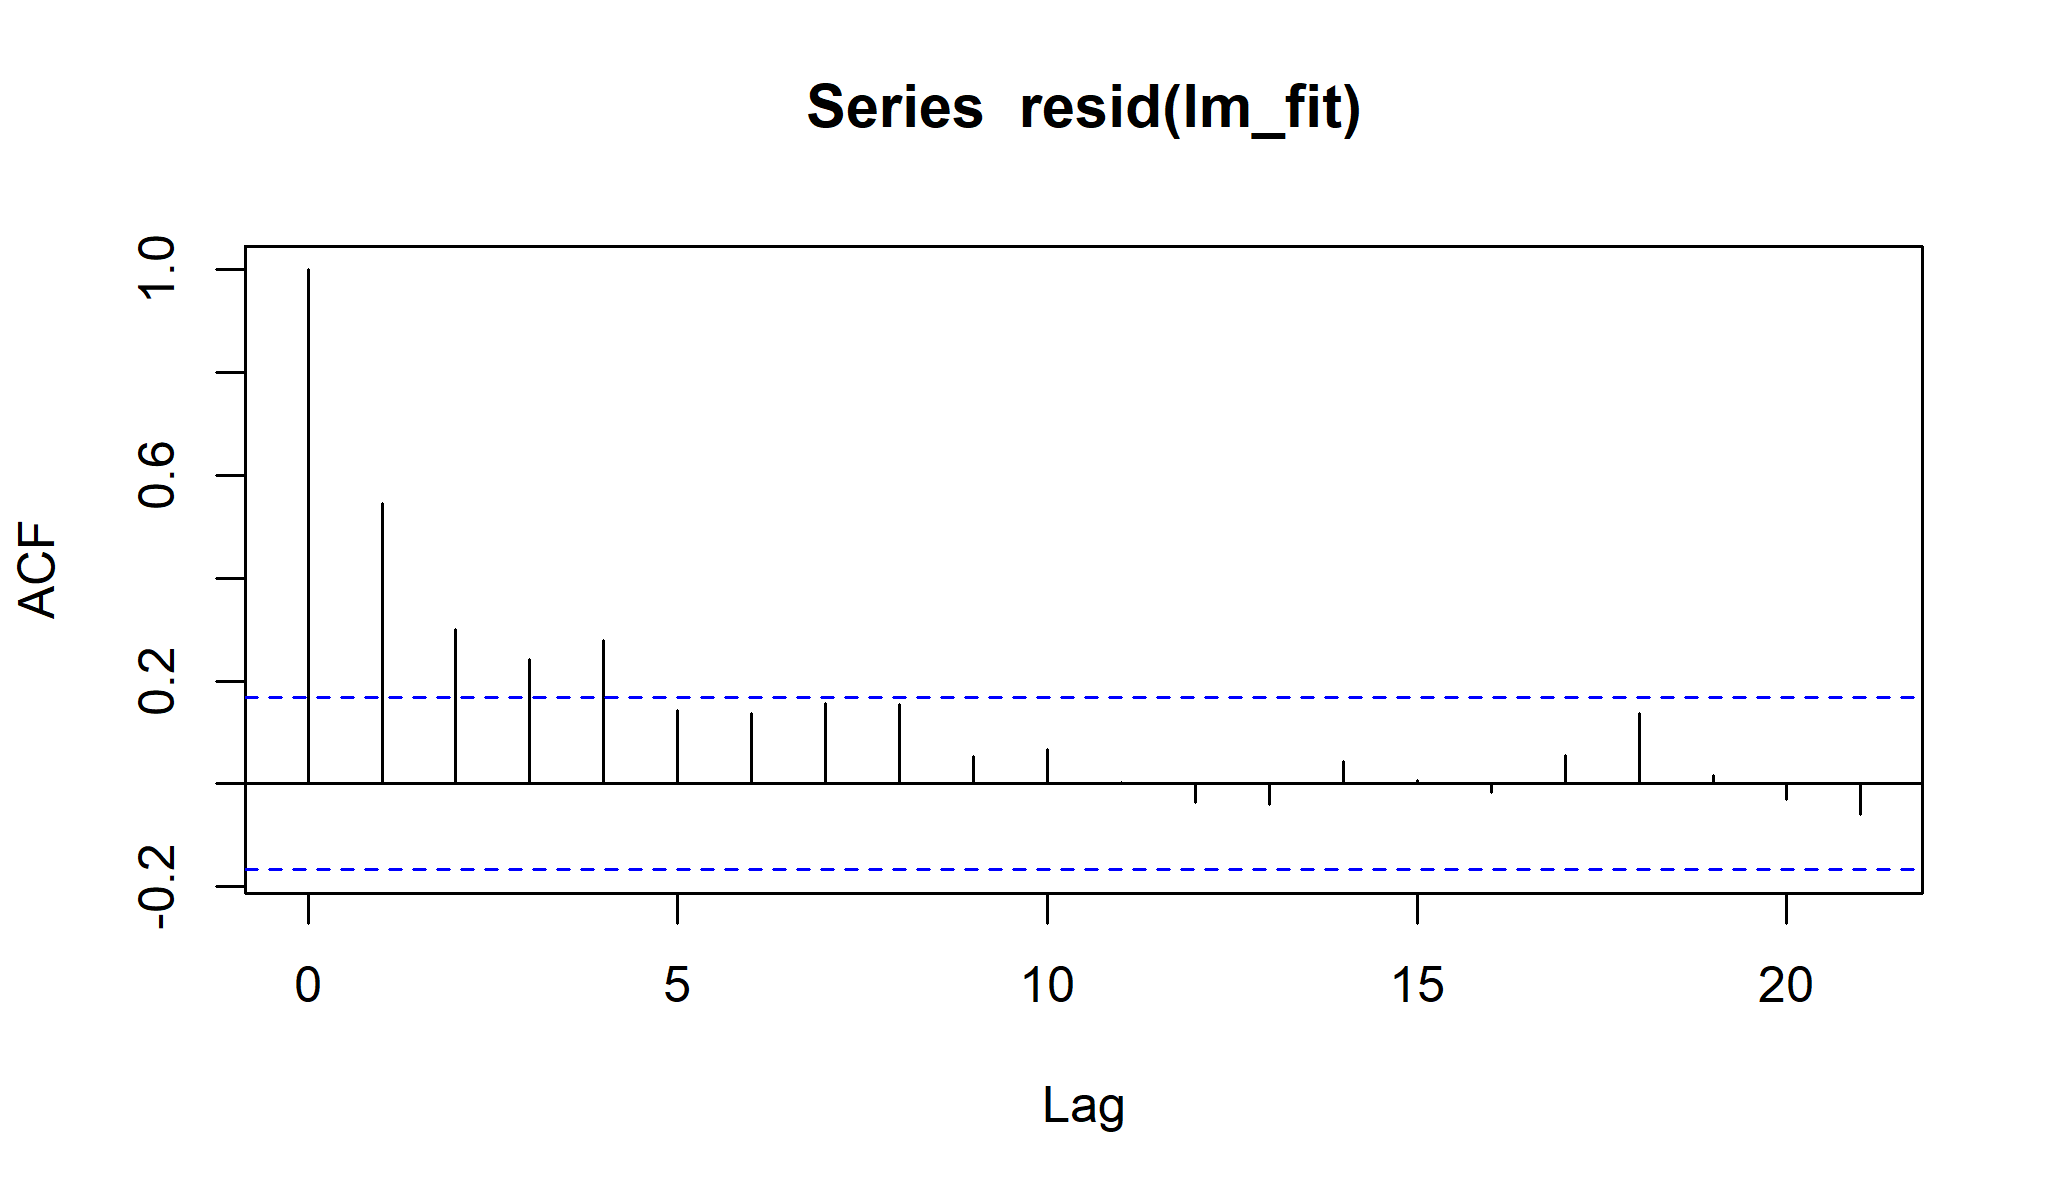
\includegraphics{figure/intro-acf_global_temp-1} \end{center}

\begin{itemize}
\item
  The horizontal \hl{dashed lines} on the graph of the sample autocorrelation
  function (ACF) give a \hl{measure of chance variation under the null
  hypothesis that the residuals are IID.}
\item
  At each lag \(h\), the chance that the estimated ACF falls within this
  band is approximately 95\%, under the null hypothesis.
\item
  Thus, \hl{under the null hypothesis, one expects a fraction of $1/20$ of
  the lags of the sample ACF to fall outside this band.}
\item
  Here, the sample ACF confirms what we can probably see from the plot
  of the fitted model: the variation around the fitted model is
  clustered in time, \hl{so the sample ACF of the residuals is not
  consistent with a model having independent error terms.}
\end{itemize}

\begin{center}\rule{0.5\linewidth}{\linethickness}\end{center}

\begin{center}\rule{0.5\linewidth}{\linethickness}\end{center}

\subsubsection{Question: How does R construct these horizontal dashed
lines?}\label{question-how-does-r-construct-these-horizontal-dashed-lines}

\begin{itemize}
\item
  Solving this question is in Homework 1.
\item
  How would you check what R actually does when it constructs these
  dashed lines? What approximation is being made? When is that
  approximation appropriate?
\end{itemize}

Hint: If you type \texttt{acf} in R, you get the source code for the acf
function. You'll see that the plotting is done by a service function
\texttt{plot.acf}. This service function is part of the package, and is
not immediately accessible to you. Nevertheless, you can check the
source code as follows

\begin{enumerate}
\def\labelenumi{\arabic{enumi}.}
\item
  Notice, either from the help documentation \texttt{?acf} or the last
  line of the source code \texttt{acf} that this function resides in the
  package \texttt{stats}.
\item
  Now, you can access this namespace directly, to list the source code,
  by

\begin{verbatim}
stats:::plot.acf
\end{verbatim}
\item
  Finally, relate this source code to the task of testing for lack of
  correlation, a standard topic in undergrad introductory statistics
  courses. The critical line of code seems to be

\begin{verbatim}
clim0 <- if (with.ci) qnorm((1 + ci)/2)/sqrt(x$n.used)
\end{verbatim}

  This appears to use a normal distribution approximation for the sample
  autocorrelation estimator, with mean zero and standard deviation
  \(1/\sqrt{N}\). Derive this approximation, for a sequence of IID mean
  zero random variables. You can ignore the issue of estimating the
  mean: suppose that the mean is known to be zero.
\end{enumerate}

\begin{center}\rule{0.5\linewidth}{\linethickness}\end{center}

\begin{center}\rule{0.5\linewidth}{\linethickness}\end{center}

\subsubsection{Generalized least
squares}\label{generalized-least-squares}

\begin{itemize}
\item
  Suppose for the moment that we knew the covariance matrix, \(\Gamma\),
  for a model with dependent errors, $${[}L2{]}
  \quad\quad\quad\quad Y = Z\beta + \zeta, \quad \quad \zeta \sim N[0,\Gamma].$$
  We read ``\(\zeta \sim N[0,\Gamma]\)'' as ``\(\zeta\) follows a
  multivariate normal distribution with mean zero and covariance matrix
  \(\Gamma\).''
\item
  The minimum variance unbiased estimator of \(\beta\) for model L2 is
  the generalized least square (GLS) estimator,
  \[\hat \beta_{GLS}(y_{1:N}) = \big( Z^{\transpose} \Gamma^{-1} Z \big)^{-1} \, Z^{\transpose} \Gamma^{-1} y.\]
\item
  The OLS estimator remains unbiased for L2 (you can check this as an
  exercise). In this sense it remains a reasonable estimator. It is
  often a practical solution to use the OLS estimator, expecially for
  preliminary data analysis. We don't know \(\Gamma\) so can't
  necessarily make a good estimator based on the GLS model. It might be
  easier to get an estimate of \(\Gamma\) once we have a reasonable
  estimate of the trend.
\item
  For model L2, the variance of the OLS estimator is
  \[\var\big[\hat \beta_{OLS}(Y_{1:N})\big] = (Z^{\transpose} Z)^{-1} \, Z^{\transpose} \Gamma Z\, (Z^{\transpose} Z)^{-1}.\]
  This is \hl{different from the variance under model L1.}
\item
  \textbf{CONCLUSION. It is okay to do ordinary linear regression for
  data which are not well modeled with uncorrelated errors. However, if
  we do so, we should not trust the error estimates coming from L1.}
  \todo[inline]{L1 will give us error estimates that are too confident}
\item
  This is an example of a situation where some parts of the output from
  statistical software are reasonable (here, the parameter estimates
  from \texttt{lm}) and other parts are unreasonable (the corresponding
  standard errors and any tests based on them). The theory helps us
  decide which bits of computer output to use and which to ignore.
\end{itemize}

\begin{center}\rule{0.5\linewidth}{\linethickness}\end{center}

\begin{center}\rule{0.5\linewidth}{\linethickness}\end{center}


\end{document}
